\documentclass[a4paper,10pt, bibliography=totocnumbered]{scrreprt}

\usepackage[utf8x]{inputenc}
\usepackage[english]{babel}

\usepackage{graphicx}
\usepackage{pdfpages}
%\usepackage{subfig}
%\usepackage{microtype}
\usepackage{tabularx}
%\usepackage{amsmath, textcomp}

% Custom packages
\usepackage[numbers]{natbib}
\usepackage{longtable}
\usepackage{ragged2e}
%\usepackage{tikz}
%\usetikzlibrary{positioning}
%\usepackage{pdflscape}
%\usepackage{rotating}

\usepackage{glossaries} 

\usepackage{hyperref}
\hypersetup{
    colorlinks=true,        % false: boxed links; true: colored links
    linkcolor=black,        % color of internal links
%    citecolor=green,        % color of links to bibliography
    citecolor=black,        % color of links to bibliography
    filecolor=magenta,      % color of file links
    urlcolor=blue           % color of external links
}


%% Title Page
\makeatletter
\renewcommand{\maketitle}{\begin{titlepage}
    \vskip 10\p@
    \hbox{
      \vrule depth 0.99\textheight
        \mbox{\hspace{2em}}
      \vtop{
        \vskip 10\p@
        \hspace{4pt}
        \vskip 50\p@
        \begin{flushleft}
          \Large \@author \par
        \end{flushleft}
        \vskip 50\p@
        \begin{flushleft}
          \huge \bfseries \@title \par
        \end{flushleft}
        \begin{flushleft}
          \Large \bfseries \@subtitle \par
        \end{flushleft}
        \vskip 70\p@
        \begin{flushleft}
          \Large \@publishers \par
        \end{flushleft}
        \vskip 50\p@
        \begin{flushleft}
          \Large \@date \par
        \end{flushleft}
        }}
  \end{titlepage}
}
\makeatother

\author{Author 1, Author n}
\title{Title }
\subtitle{Technical Report}
\publishers{\textbf{Advisor University of Heidelberg}\\ Prof. Dr. Barbara Paech, Michael Anders}
\date{mm dd, year}



% Deutsche Absaetze:
\parindent 0pt
\parskip 12pt

\textwidth145mm
\setlength{\oddsidemargin}{0.7cm}
\setlength{\topmargin}{-0.5cm}
\setlength{\textheight}{22.5cm}

\begin{document}
\maketitle

\begin{abstract}
\section*{Abstract}
Place the abstract in this section.
\end{abstract}

\tableofcontents

\chapter{Introduction}
Lorem ipsum dolor sit amet, consectetuer adipiscing \textbf{Figure \ref{fig:model}} elit. Vivamus elementum sem eget tortor. Pellentesque id orci cursus sem tempus porttitor. Aenean tincidunt, neque vitae bibendum lacinia, magna erat dapibus nunc, vel pharetra nibh erat ac lorem. Ut suscipit ante eget magna. Morbi luctus aliquet odio. 

\section{Subsection}
Aenean turpis velit, ullamcorper sed, viverra vel, consectetuer sit amet, \cite{KunChen2005} Chenipsum. Phasellus sed lectus. Vivamus fermentum odio sed odio. Donec a dui. Duis et neque quis ligula pulvinar porttitor. Nunc mattis lectus vitae diam. 

Praesent quis orci. Aliquam id urna. Sed dolor erat, faucibus et, mattis eget, \textbf{commodo} nec, lorem. Etiam sit amet nisi sit amet nisi posuere bibendum. \emph{Cum sociis natoque} penatibus et magnis dis parturient montes, nascetur ridiculus mus. 


\begin{figure}
\centering
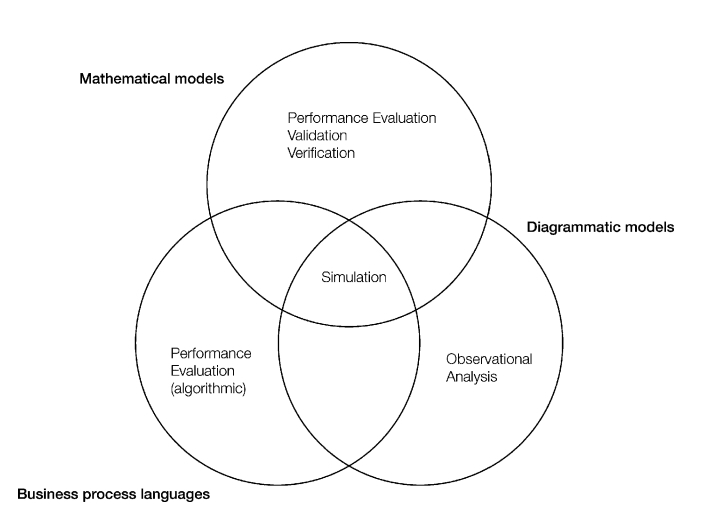
\includegraphics[scale=0.65]{images/T1Figure01.pdf} 
\caption{caption text}
\label{fig:model}
\end{figure}

\begin{itemize}
\item Aliquam
\item mus
\item montes
\end{itemize}

\subsubsection{Subsubsection}
Lorem ipsum dolor sit amet, consectetuer adipiscing elit. Vivamus elementum sem eget tortor. Pellentesque id orci cursus sem tempus porttitor. Aenean tincidunt, neque vitae bibendum lacinia, magna erat dapibus \textbf{Table \ref{tab:table}} nunc, vel pharetra nibh erat ac lorem. Ut suscipit ante eget magna. Morbi luctus aliquet odio. Aenean turpis velit, ullamcorper sed, viverra vel, 

 \begin{table} [t] 
\centering
\begin{small}
\caption{Table caption text}
\label{tab:table}
\setlength{\tabcolsep}{1em}
\begin{tabular}{ l| p{8cm}}
\hline
 \textbf{X} & \textbf{ Y} \\
\hline
 \hline	
 Item1 & description\\
 \hline
  Item2 & description  \\
 \hline
  Item2 & description \\
 \hline
\end{tabular}
\end{small}
\end{table}

\chapter{Richtiges Zitieren}

1.	Die Seminararbeit ist eine eigenständige wissenschaftliche Arbeit und wird auch nach den Regeln einer wissenschaftlichen Arbeit erstellt (vgl.~\cite{RichtigesZitierenTUDresden}), insbesondere heißt das, dass die Regeln für:
\begin{enumerate}
\item Richtiges Zitieren 
\begin{itemize}
\item Zitierpflicht
\item Zitierregeln
\item Typen von Zitaten
\item Zitierformen
\end{itemize}
\item Literaturangaben 
\item eine gut strukturierte Arbeit 
\end{enumerate}
beachtet und eingehalten werden.




\chapter{Chapter}

Duis porta orci. Integer eu arcu at enim tempus facilisis. Pellentesque dignissim orci sed est. Etiam elementum laoreet mi. Donec nunc sapien, dictum in, tristique sed, aliquam vitae, massa. Morbi magna magna, vestibulum tempor, lobortis non, convallis nec, nibh. In sed nibh. Suspendisse adipiscing dictum pede. Suspendisse non augue. Lorem ipsum dolor sit amet, consectetuer adipiscing elit. Pellentesque lacinia, velit sed commodo convallis, diam dolor consequat ligula, a scelerisque quam neque et purus. Praesent vel augue. Sed lectus leo, dignissim eget, vulputate eu, auctor ut, nulla. Vivamus a quam. Nulla tellus. Pellentesque tempor pulvinar nunc.


% !TeX spellcheck = en_US
\chapter{Problem Classification in Bug Tracking Systems}

\section{Introduction}

The goal of this topic is to classify issues in Bug Tracking Systems (BTS). Issues can be classified into various categories depending on the topics they address and their type or they can be classified into different levels of importance, in which case we talk about prioritization. BTS are used as an organizational tool for developers and a feedback pipeline for users. While the original purpose of those systems is to manage bug issues, they can and are used for many different kinds of issues not related to corrective maintenance as well \cite{Antoniol2008}. Because of the many different kinds of issues it is of interest to sort those issues by type and priority. As the amount of issues is ever increasing the approaches discussed in this chapter aim to automate this classification process to save time and resources.\\
The articles ''Is it a Bug or an Enhancement? A Text-based Approach to Classify Change Requests'' by Antoniol \textit{et al.} \cite{Antoniol2008} and ''CaPBug-A Framework for Automatic Bug Categorization and Prioritization Using NLP and Machine Learning Algorithms'' by Ahmed \textit{et al.} \cite{Ahmed2021} are investigated. Antoniol \textit{et al.} aim to classify BTS issues into bugs and non-bugs and Ahmed \textit{et al.} propose a framework to classify bugs into six bug types and prioritize bugs into five levels.\\
In the next section a literature search used to identify the article by Ahmed \textit{et al.} based on the given article by Antoniol \textit{et al.} and the topic is outlined. The research question and relevance criteria used for the search are introduced. The search involves snowballing as well as a term-based search. The following two sections describe the two approaches in detail. They contain subsections about the goals, algorithms, evaluate the approaches and give examples of how a bug issue is preprocessed. In the fifth section the articles are compared to each other based on a series of synthesis questions. Lastly a short conclusion is drawn.\\
For clarification on requirements engineering, natural language processing or machine learning terms used and tools referenced in this chapter, please refer to the glossary.

\section{Literature Search}
The research question on which the literature search was based is ''How, into which classes and with what quality can Bug Tracking System Issues be classified?''. This question addresses out interest in the different algorithms used, the classification goals and the quality of the approaches.\\
To filter potential literature the following criteria of relevance were introduced:
\begin{itemize}
\item The goal of the algorithm must be to classify issues.
\item These issues must stem from Bug Tracking Systems (BTS).
\item The article must be available in German or English language.
\item The article must not be from the same authors as the already provided article \cite{Antoniol2008}.
\item The article must not be older than ten years, ideally less than five.
\end{itemize}

For the literature search forward and backward snowballing and a term-based search were used. Antoniol \textit{et al.} references 25 articles and is referenced by 208. As Antoniol \textit{et al.} is from 2008 none of the articles it references fit the relevance criteria. Of the referencing articles, ''Predicting issue types on GitHub'' by Kallis \textit{et al.} \cite{Kallis2021}, a publication from 2021 in which the tool ''ticket tagger'' for classifying GitHub issues is proposed, was identified as a potential candidate for a second approach.\\
The term-based search was performed in IEEE \cite{IEEE} and ACM \cite{ACM}, which contain a big repertoire of information technology related articles by trustworthy sources. Individual searches were performed as presented in \mbox{Table \ref{tab:LitSearch}}. As search terms (''Bug Tracking'' OR ''Bug Report'') was used to select articles that are concerned with BTS as issue source and (''Classification'' OR ''Identification'') was used so articles would have classification as a goal.\\

\begin{table} [h] 
\centering
\begin{footnotesize}
\setlength{\tabcolsep}{0.3em}
\renewcommand{\arraystretch}{1.5}
\caption{Term-based search for Problem Classification in Bug Tracking Systems}
\label{tab:LitSearch}
\begin{tabular}{l| p{0.7cm}|p{1.8cm}|p{2.2cm}|p{1.2cm}|p{1.5cm}|p{1.5cm}|p{3cm}}
\hline
\textbf{Source} & \textbf{Date} & \textbf{Restrictions} & \textbf{Searchterms} & \textbf{\#results} & \textbf{\#relevant results} & \textbf{\#relevant new \mbox{results}} & \textbf{further used \mbox{results}} \\ [0.5ex] 
\hline	
\hline	
  ACM & 08.11. 2021 & - & ("Bug Tracking" OR "Bug Report") AND ("Classification" OR "Identification") & 1076 & 1 in first 50 & 1 & -\\[0.5ex]
\hline	
ACM & 08.11. 2021 & not older than 5 years & ("Bug Tracking" OR "Bug Report") AND ("Classification" OR "Identification") & 384 & 5 in first 50 & 3 & Otoom \textit{et al.}, "Automated Classification of Software Bug Reports", ICICM, 2019\\[0.5ex]
\hline	
ACM & 08.11. 2021 & not older than 5 years, Abstract only & ("Bug Tracking" OR "Bug Report") AND ("Classification" OR "Identification") & 11 & 2 & 0 & - \\
\hline	
IEEE & 08.11. 2021 & 2016 onwards &  "Bug Report" AND "Classification" & 52 & 3 & 1 & Ahmed \textit{et al.}, "CaPBug - A Framework for Automatic Bug Categorization and Prioritization Using NLP and Machine Learning Algorithms", IEEE Access, 2021\\
\hline
\end{tabular}
\end{footnotesize}
\end{table}

The term-based search yielded ''Automated classification of software bug reports'' by Otoom \textit{et al.} \cite{Otoom2019}, an article from 2019 separating corrective and perfective issues with high accuracy, and ''CaPBug-A Framework for Automatic Bug Categorization and Prioritization Using NLP and Machine Learning Algorithms'' by Ahmed \textit{et al.} \cite{Ahmed2021}, an article from 2021 presenting CaPBug, a tool to prioritize Bugs and classify them into six categories, as potential second approach to be investigated.\\
To decide which approach to investigate, the three candidates were compared in \mbox{Table \ref{tab:LitComp}}. Criteria were the recency of the articles, the quality of the classification, the nature of the algorithm and classification goals. The aim is to find a second article that answers the research question, but gives a different answer than Antoniol \textit{et al.}. Ahmed \textit{et al.} was chosen mainly because of its different classification goal. The other articles were more similar to Antoniol \textit{et al.} in their algorithm as well as their classification goals.

\begin{table} [h] 
\centering
\begin{small}
\setlength{\tabcolsep}{1em}
\caption{Comparison of candidates for second article.}
\label{tab:LitComp}
\begin{tabular}{ p{5cm}| p{2cm}|l}
\hline
 \textbf{Article} & \textbf{ Source} & \textbf{Pros and Cons}\\
\hline
 \hline	
  \textit{Kallis et al.}, "Predicting issue types on GitHub", Science of Computer Programming 205, 2021 &Forward-Snowballing & \thead[l]{\textcolor{blue}{+ Very recent}\\ \textcolor{blue}{+ Großes Datenset} \\ \textcolor{red}{- Similar to Antoniol et al.}}\\
 \hline
  \textit{Otoom et al.}, "Automated Classification of Software Bug Reports", ICICM, 2019 & ACM Search & \thead[l]{\textcolor{blue}{+ Recent}\\ \textcolor{blue}{+ high accuracy} \\ \textcolor{red}{- Very similar to Antoniol et al.}}\\
 \hline
  \textit{Ahmed et al.}, "CaPBug - A Framework for Automatic Bug Categorization and Prioritization Using NLP and Machine Learning Algorithms", IEEE Access, 2021 & IEEE Search & \thead[l]{\textcolor{blue}{+ Very recent} \\ \textcolor{blue}{+ Very thorough} \\ \textcolor{blue}{+ many classes} \\ \textcolor{blue}{+ different classification goal than}\\ \textcolor{blue}{Antoniol et al.}}\\
 \hline
\end{tabular}
\end{small}
\end{table}

\section{Approach 1: Is it a Bug or an Enhancement? A Text-based Approach to Classify Change Requests}
\subsection{Goal}
In their article ''Is it a Bug or an Enhancement? A Text-based Approach to Classify Change Requests'' Antoniol \textit{et al.} address the problem that Bug Tracking Systems (BTS) contain various types of issues, bugs, enhancement requests and organizational issues among others. In the dataset used, only about one third (Eclipse) to about 78\% (JBoss) of issues were found to be actual bugs. The approach described in the article classifies issues automatically into bugs and non-bugs by using machine learning classifiers. The authors pose the research questions: \begin{itemize}
\item RQ1: To what extend can issue information be used to distinguish bugs and non-bugs?
\item RQ2:  What are the terms/fields that machine learning models use to discern bugs from other issues?
\item RQ3: Does the approach perform better than classification by regular expression matching?
\end{itemize}

\subsection{Algorithm}
Input for the algorithm are 600 randomly chosen BTS issues labeled ''resolved'', ''verified'' or ''closed'' each from Eclipse, Mozilla and JBoss. For the Oracle three developers decide with simple majority if an issue is a bug, a non-bug (non-corrective maintenance) or something other.\\
The linguistic features from the title, issue description and discussion are preprocessed using text filtering, stemming and indexing. In filtering, the punctuation was removed and paths are split. For stemming, the Porter stemmer from the \textit{lsa} package of R was used to remove plurals and break down verbs to their infinitive. Antoniol \textit{et al.} chose not to use stopping as they suspect that common words such ''should'', ''might'' and ''not'' can be important to identify bugs. For indexing they use the raw word frequency instead of the common TF-IDF, so common but important terms such as ''failure'' and ''crash'' are not penalized. The authors report only results for features from the description only, as this gives the best classification results.\\
For automatic classification the authors used \textit{Weka} tool.
They use an unnamed feature selection algorithm to select a subset of the available features and then train different classifiers, naive Bayes, alternating decision trees and linear logistic regression, to classify the issues. 10-fold cross validation is used.

\subsection{Evaluation}
The accuracy of the classification, compared to the Oracle, using different classifiers are shown in \mbox{Table \ref{tab:Antoniol}}. The values for Mozilla and Eclipse are obtained with the 50 best features used and the ones with JBoss with the best 100. Using less features gave lower accuracy and using more features did, according to the authors, not further improve accuracy.\\
The best accuracy for classification was reached using  the linear logistic regression classifier. In Mozilla, issues were correctly labeled 77\% of the time and in Eclipse and JBoss the accuracy was 82\%.
\\
The authors report that terms such as ''crash'', ''critic'', ''broken'' and ''when'' indicate a bug, while ''should'', ''implement'' and ''support'' lead to non-bug classifications. Note that the terms ''when'' and ''should'' would have been removed by stopping.
\\ 
As seen in \mbox{Table \ref{tab:Antoniol}} automatic classification with machine learning classifiers outperformed regular expression search with \textit{grep} for all used classifiers and data.
\\
The research of Antoniol \textit{et al.} shows that BTS issues can be classified quite well into bugs and non-bugs. In terms of practical application the question remains how the issues labeled ''other'' by the oracle would be classified by the algorithm and how one would distinguish those from bugs.
\begin{table} [h] 
\centering
\setlength{\tabcolsep}{1em}
\renewcommand{\arraystretch}{1.5}
\caption{Accuracy for classification using different classifiers or regular expression search (grep)}
\label{tab:Antoniol}
\begin{tabular}{p{1cm}|p{2cm}|p{3cm}|p{4cm}|p{0.8cm}}
\hline
 \textbf{Quelle} & \textbf{with naive Bayes}& \textbf{with alternating decision trees}&\textbf{with logistic regression} &  \textbf{grep}\\
\hline
 \hline
Mozilla & 72\% & 68\% & 77\% & 46\% \\
 \hline
Eclipse & 81\% & 79\% & 82\% & 67\% \\
 \hline
JBoss & 54\% & 76\% & 82\% & 39\%\\
 \hline
\end{tabular}
\end{table}

\subsection{Example}
To be done.

\section{Approach 2: CaPBug - A Framework for Automatic Bug Categorization and Prioritization Using NLP and Machine Learning Algorithms}

\subsection{Goal}
Bugs, their priority and category play a big role in software maintenance and development. In their article  ''CaPBug - A Framework for Automatic Bug Categorization and Prioritization Using NLP and Machine Learning Algorithms'' Ahmed \textit{et al.} aim to reduce the resources needed to manage bug issues by automating classification and prioritization. They propose a framework CapBug, which stands for Categorization and Prioritization of Bugs, that both classifies and prioritizes issues, while other articles focus on one or the other. The categories for the classification are ''Program Anomaly'', ''GUI'', ''Network or Security'', ''Configuration'', ''Performance'' and ''Test Code'' and they distinguish between five levels of priority.\\
Results obtained using different machine learning classifiers and textual or linguistic features are compared and for prioritization the effect of SMOTE is investigated.

\subsection{Algorithm}
The source for the BTS issues are Bugzilla repositories for Eclipse and Mozilla. Ahmed \textit{et al.} used keyword search to identify issues for each category and 
To be done.

\subsection{Evaluation}
To be done.

\subsection{Example}
To be done.

\section{Comparison}
\subsection{Antoniol \textit{et al.}}
The approach of the article "Is it a Bug or an Enhancement? A Text-based Approach to
Classify Change Requests" \cite{Antoniol2008} will be referred to as "Antoniol \textit{et al.}", as the authors don't give a name to their classification system.\\
For this approach supervised machine learning is used to classify bug issues into bugs and non-bugs (other activities). Decision trees, naive Bayes classifier and logistic regression were used as classifiers. Linguistic features (terms in the description) undergo text filtering, stemming, and indexing before being used. Fields (e.g. severity) of the bug tracking systems are also used. An unnamed feature selection algorithm is used to select a subset of available features.\\
For training issues are manually classified into bugs and non-bugs (three developers, simple minority). The bug tracking systems for Mozilla, Eclipse and JBoss were used as targets.\\
This approach helps with software maintenance, as it allows to extract bug issues from bug tracking systems. Supported stakeholders are developers, especially those tasked with maintenance and quality control.\\
There is no single tool to use this approach. Feature extraction is done using Pearl and R scripts, and automatic classification was done using Weka tool.\\
Performance was evaluated using 10-fold cross validation. Results for 20 and 50 features for Mozilla and Eclipse and 50 and 100 features for JBoss are shown in the article. The number of issues for each predicted label - actual label, the precision, recall and percentage of correct decisions are shown for each classifier and each bug tracking system.\\
The approach reaches the best accuracy of 77\% in the Eclipse and 82\% in the other datasets with linear logistic regression classifier and performs better than regex search for all classifiers.

\subsection{CaPBug}
The authors call their framework used in the article "CaPBug - A Framework for Automatic Bug Categorization and Prioritization Using NLP and Machine Learning Algorithms" \cite{Ahmed2021} CaPBug.\\
CaPBug uses textual features (summary attribute of the issues with natural language processing (NLP) applied) as well as categorical features (component, assignee, status, priority, category...) for classification. The datasets are categorized into the categories Program Anomaly, GUI, Network or Security, Configuration, Performance, and Test-Code and five different priority levels. For NLP, tokenization, stop words removal and lemmatization are used and Term Frequency-Inverse Document Frequency
(TF-IDF) is used for feature extraction. To balance the classes (categories) CaPBug uses Synthetic Minority Oversampling Technique (SMOTE).\\
The datasets are divided into 80\% training and 20\% testing data. For machine learing classification algorithms Naive Bayes, Random Forest, Decision Trees and Logistic Regression are used.\\
This approach helps in the maintenance and quality control tasks of software developers by classifying and prioritizing bugs. \\
For NLP the Python Natural Language Processing Toolkit (NLTK) is used. Other than that it is not described what tools are used.\\
Results for CaPBug with textual or categorical features, for classification or prioritization, with or without SMOTE for the four different ML classifiers are reported. Precision, Recall, Accuracy and f1-score are used for evaluation.\\
The textual feature is more useful for classification and prioritization than categorical features and random forest is the best performing classifier (88.78\% accuracy for category prediction and 90.43\% with SMOTE for priority).

\subsection{Differences and Similarities}

The approaches are compared in the synthesis matrix shown in \mbox{Table \ref{tab:Synthesis}}.\\

\begin{table} [h] 
\centering
\begin{small}
\caption{Synthesis matrix for Problem Classification in Bug Tracking Systems}
\label{tab:Synthesis}
\setlength{\tabcolsep}{1em}

\renewcommand{\arraystretch}{1.5}
\begin{tabular}{ l| p{2.5cm}|p{4.4cm}|p{4.4cm}}
\hline
 \textbf{Nr.} & \textbf{ Name} & \textbf{Antoniol \textit{et al.} \cite{Antoniol2008}}& \textbf{CaPBug-A Framework \cite{Ahmed2021}}\\
\hline
 \hline	
 3a) & Methods used& Decision trees, naive Bayes classifier, logistic regression& TF-IDF, SMOTE, Decision trees, naive Bayes, logistic regression, random forest\\
 \hline
  3b) & Classification goal  & bug vs. non-bug & Categories: Program Anomaly, GUI, Network or Security, Configuration, Performance, and Test-Code ; 5 priority levels\\
 \hline
  3c) & Prerequisites and restrictions of data and approach & Oracle (classified data for training) & Bug issues for different categories identified by keyword search; class imbalance (addressed by SMOTE)\\
 \hline
4a) & Supported development processes & Maintenance, quality control& Maintenance, quality control\\
 \hline
4b) & Supported stakeholders & Software developers & Software developers \\
 \hline
5a) & Supported tools / Prototypes & none & none\\
 \hline
5b) & Degree of automation & medium; Pearl Script for feature extraction, \textit{Weka} tools for classification & low\\
 \hline
6a) & Evaluation of approach & precision, recall, accuracy, comparison to regex search & precision, recall, accuracy, f1-score\\
 \hline
6b) & Important evaluation results & classification with linear regression has best accuracy of 77-82\% (depending on dataset), outperforms regex search for all classifiers& Random Forest with textual features gives best accuracy of 88.78\% for classification and with SMOTE 90.43\% for prioritization, SMOTE improves prioritization\\
 \hline
\end{tabular}
\end{small}
\end{table}

While both approaches aim to classify bug issues, CaPBug also prioritizes the bugs. Antoniol \textit{et al.} uses a random subset of closed issues from bug tracking systems, while CaPBug selects issues randomly from the ones that match their categories (keyword search is part of this selection process). CaPBug also says that only "real flaws", so issues that would be classified as bug by Antoniol \textit{et al.}, are used. The sources of issues are comparable for both approaches, both use the Bugzilla for Eclipse amongst others.\\
For pre-processing different NLP methods are used. For example Antoniol \textit{et al.} does explicitly not use stopping because terms like "should", "might" and "not" carry important information in their context, while CaPBug uses stopping. For feature extraction TF-IDF is used by CaPBug, while "Is it a Bug or an Enhancement?" uses raw frequency, as for their problem common terms such as "failure" should not be penalized. CaPBug uses SMOTE for class balancing, while Antoniol \textit{et al.} does not attempt class balancing. For machine learning classifiers both use naive bayes, decision trees and logistic regression, while CaPBug also uses random forest.\\
Both approaches, the classification into bugs and non-bugs and the classification into different types of bugs, achieve high accuracy.

\section{Conclusion}

Bug tracking systems are important tools for software maintenance and development. They contain issues of different nature and priority. To save resources these issues can automatically be classified and prioritized using natural language processing and machine learning classifiers.\\
Antoniol \textit{et al.} showed that BTS issues can be divided into bug and non-bug issues with high accuracy. Ahmed \textit{et al.} showed that bugs can accurately be further divided into categories, which can help resource allocation. They furthermore showed that bugs can accurately be prioritized when using SMOTE.\\
Both approaches make restrictions during the selection of issues used for their classification, which introduces uncertainty how well the approaches would work on unfiltered data.


%\section{Summary}
%The issue addressed in the article "Is it a Bug or an Enhancement? A Text-based Approach to Classify Change Requests" \cite{Antoniol2008} by Antoniol \textit{et al.} is that bug tracking systems contain true bugs, which are defined as issues of corrective maintenance, as well as other issues. They are among the first to try to automatically classify issues into these categories by using supervised machine learning (native bayes, decision tree and logistic regression). They manage to distinguish bugs and non-bugs with an accuracy of up to 82\%, much better than the accuracy of a regex-search approach.\\
%In "CaPBug - A Framework for Automatic Bug Categorization and Prioritization Using NLP and Machine Learning Algorithms" Ahmed \textit{et al.} aim to automatically categorize and prioritize bug issues simultaneously, as previous research mainly focused on the problems independently. They provide a framework for categorization into six different categories and prioritization into five levels. The different machine learning categorizers (naive bayes, decision trees, logistic regression and random forest), two types of features (textual and categorical) and the use of SMOTE for class balancing are evaluated. The research finds that a random forest classifier with textual features (that is features extracted from the summary by natural language processing) works best with an accuracy of 88.78\% for category and 90.43\% for priority prediction.
%
%\section{Synthesis}
%\subsection{Is it a Bug or an Enhancement?}
%\subsubsection{1 - Name of the approach}
%The approach of the article "Is it a Bug or an Enhancement? A Text-based Approach to
%Classify Change Requests" \cite{Antoniol2008} will be referred to as "Is it a Bug or an Enhancement?", as the authors don't give a name to their classification system.
%\subsubsection{3 - Description}
%For this approach supervised machine learning is used to classify bug issues into bugs and non-bugs (other activities). Decision trees, naive Bayes classifier and logistic regression were used as classifiers. Linguistic features (terms in the description) undergo text filtering, stemming, and indexing before being used. Fields (e.g. severity) of the bug tracking systems are also used. An unnamed feature selection algorithm is used to select a subset of available features.\\
%For training issues are manually classified into bugs and non-bugs (three developers, simple minority). The bug tracking systems for Mozilla, Eclipse and JBoss were used as targets.
%\subsubsection{4 - Uses}
%This approach helps with software maintenance, as it allows to extract bug issues from bug tracking systems. Supported stakeholders are developers, especially those tasked with maintenance and quality control.
%\subsubsection{5 - Tool support}
%There is no single tool to use this approach. Feature extraction is done using Pearl and R scripts, and automatic classification was done using Weka tool.
%\subsubsection{6 - Evaluation}
%Performance was evaluated using 10-fold cross validation. Results for 20 and 50 features for Mozilla and Eclipse and 50 and 100 features for JBoss are shown in the article. The number of issues for each predicted label - actual label, the precision, recall and percentage of correct decisions are shown for each classifier and each bug tracking system.\\
%The approach classifies up to 82\% of issues correctly into bugs and non-bugs and performs better than regex search across the board.
%
%\subsection{CaPBug}
%\subsubsection{1 - Name of the approach}
%The authors call their framework used in the article "CaPBug - A Framework for Automatic Bug Categorization and Prioritization Using NLP and Machine Learning Algorithms" \cite{Ahmed2021} CaPBug.
%\subsubsection{3 - Description}
%CaPBug uses textual features (summary attribute of the issues with natural language processing (NLP) applied) as well as categorical features (component, assignee, status, priority, category...) for classification. The datasets are categorized into the categories Program Anomaly, GUI, Network or Security, Configuration, Performance, and Test-Code and five different priority levels. For NLP, tokenization, stop words removal and lemmatization are used and Term Frequency-Inverse Document Frequency
%(TF-IDF) is used for feature extraction. To balance the classes (categories) CaPBug uses Synthetic Minority Oversampling Technique (SMOTE).\\
%The datasets are divided into 89\% training and 20\% testing data. For machine learing classification algorithms Naive Bayes, Random Forest, Decision Trees and Logistic Regression are used.
%\subsubsection{4 - Uses}
%This approach helps in the maintenance and quality control tasks of software developers by classifying and prioritizing bugs. 
%\subsubsection{5 - Tool support}
%For NLP the Python Natural Language Processing Toolkit (NLTK) is used. Other than that it is not described what tools are used.
%\subsubsection{6 - Evaluation}
%Results for CaPBug with textual or categorical features, for classification or prioritization, with or without SMOTE for the four different ML classifiers are reported. Precision, Recall, Accuracy and f1-score are used for evaluation.\\
%The textual feature is more useful for classification and prioritization than categorical features and random forest is the best performing classifier (88.78\% accuracy for category prediction and 90.43\% for priority).
%\pagebreak
%\section{Synthesis Matrix}
%\begin{table} [h] 
%\centering
%\begin{small}
%\caption{Synthesis matrix for Problem Classification in Bug Tracking Systems}
%\label{tab:table}
%\setlength{\tabcolsep}{1em}
%\begin{tabular}{ l| p{3cm}|p{5cm}|p{5cm}}
%\hline
% \textbf{Nr.} & \textbf{ Name} & \textbf{Is it a Bug or an Enhancement? \cite{Antoniol2008}}& \textbf{CaPBug-A Framework \cite{Ahmed2021}}\\
%\hline
% \hline	
% 3a) & Methods used& Decision trees, naive Bayes classifier, logistic regression& TF-IDF, SMOTE, Decision trees, naive Bayes, logistic regression, random forest\\
% \hline
%  3b) & Classification goal  & bug vs. non-bug & Categories: Program Anomaly, GUI, Network or Security, Configuration, Performance, and Test-Code ; 5 priority levels\\
% \hline
%  3c) & Prerequisites and restrictions of data and approach & Oracle (classified data for training) & Bug issues for different categories identified by keyword search; class imbalance (addressed by SMOTE)\\
% \hline
%4a) & Supported development processes & Maintenance, quality control& Maintenance, quality control\\
% \hline
%4b) & Supported stakeholders & software developers &software developers \\
% \hline
%5a) & Supported tools / Prototypes & Pearl, R, Weka tools& Python NLTK\\
% \hline
%5b) & Degree of automation & low & low\\
% \hline
%6a) & Evaluation of approach & precision, recall, accuracy, comparison to regex search & precision, recall, accuracy, f1-score\\
% \hline
%6b) & Important evaluation results & classifies issues with up to 82\% accuracy, outperforms regex search& classifies issues with up to 88.78\% and prioritizes with up to 90.43\% accuracy\\
% \hline
%\end{tabular}
%\end{small}
%\end{table}
%
%\section{Differences and Similarities}
%
%While both approaches aim to classify bug issues, CaPBug also prioritizes the bugs. "Is it a Bug or an Enhancement?" uses a random subset of closed issues from bug tracking systems, while CaPBug selects issues randomly from the ones that match their categories (keyword search is part of this selection process). CaPBug also says that only "real flaws", so issues that would be classified as bug by "Is it a Bug or an Enhancement?", are used. The sources of issues are comparable for both approaches, both use the Bugzilla for Eclipse amongst others\\
%For pre-processing different NLP methods are used. For example does "Is it a Bug or an Enhancement?" explicitly not use stopping because terms like "should", "might" and "not" carry important information in their context, while CaPBug uses stopping. For feature extraction TF-IDF is used by CaPBug, while "Is it a Bug or an Enhancement?" uses raw frequency, as for their problem common terms such as "failure" should not be penalized. CaPBug uses SMOTE for class balancing, while "Is it a Bug or an Enhancement?" does not attempt class balancing. For machine learning classifiers both use naive bayes, decision trees and logistic regression, while CaPBug also uses random forest.\\
%Both approaches, the classification into bugs and non-bugs and the classification into different types of bugs, achieve high accuracy.




\chapter{Conclusion}
Fusce vitae quam eu lacus pulvinar vulputate. Suspendisse potenti. Aliquam imperdiet ornare nibh. Cras molestie tortor non erat. Donec dapibus diam sed mauris laoreet volutpat. Sed at ante id nibh consectetuer convallis. Suspendisse diam tortor, lobortis eget, porttitor sed, molestie sed, nisl. Integer enim nisl, lacinia in, pretium eu, viverra a, odio. Quisque at quam eget risus placerat porttitor. Suspendisse convallis, elit vitae mattis pharetra, orci nisl ultrices sapien, ac interdum metus lorem iaculis diam. Nunc id nunc sit amet nisl tincidunt congue. Curabitur et sapien.

%% Bibliography
\bibliographystyle{plainnat}
%\bibliography{literature.bib}%Bibliography file name

\begin{thebibliography}{9}

\bibitem{KunChen2005} Chen, K, Zhang, W., Zhao, H.: An approach to constructing feature models based on requirements clustering.
In: 13th IEEE International Conference on Requirements Engineering (RE05). pp. 31-40. (2005)

\bibitem{RichtigesZitierenTUDresden} Institut für Geographie   
Lehrstuhl für Allgemeine Wirtschafts- und Sozialgeographie: An Hinweise zum wissenschaftlichen Arbeiten.
\url{http://www.geogr.uni-jena.de/fileadmin/Geoinformatik/Lehre/backup_05_2007/pdf-dokumente/Skript_WissArbeiten.pdf}

% Sources Topic 2 Start
\bibitem{Ciurumelea.2017} A. Ciurumelea, A. Schaufelbühl, S. Panichella and H. C. Gall, "Analyzing reviews and code of mobile apps for better release planning" 2017 IEEE 24th International Conference on Software Analysis, Evolution and Reengineering (SANER), 2017, pp. 91-102, doi: 10.1109/SANER.2017.7884612.
  
\bibitem{Scalabrino.2019} S. Scalabrino, G. Bavota, B. Russo, M. D. Penta and R. Oliveto, "Listening to the Crowd for the Release Planning of Mobile Apps," in IEEE Transactions on Software Engineering, vol. 45, no. 1, pp. 68-86, 1 Jan. 2019, doi: 10.1109/TSE.2017.2759112.

\bibitem{Villarroel.2016}L. Villarroel, G. Bavota, B. Russo, R. Oliveto and M. Di Penta, "Release Planning of Mobile Apps Based on User Reviews," 2016 IEEE/ACM 38th International Conference on Software Engineering (ICSE), 2016, pp. 14-24, doi: 10.1145/2884781.2884818.
  
\bibitem{Mahmud.2019}O. Mahmud, N. T. Niloy, M. A. Rahman and M. S. Siddik, "Predicting an Effective Android Application Release Based on User Reviews and Ratings," 2019 7th International Conference on Smart Computing \& Communications (ICSCC), 2019, pp. 1-5, doi: 10.1109/ICSCC.2019.8843677.

\bibitem{Noei.2019}E. Noei, F. Zhang and Y. Zou, "Too Many User-Reviews! What Should App Developers Look at First?," in IEEE Transactions on Software Engineering, vol. 47, no. 2, pp. 367-378, 1 Feb. 2021, doi: 10.1109/TSE.2019.2893171.

\bibitem{Aslam.2020}N. Aslam, W. Y. Ramay, K. Xia and N. Sarwar, "Convolutional Neural Network Based Classification of App Reviews," in IEEE Access, vol. 8, pp. 185619-185628, 2020, doi: 10.1109/ACCESS.2020.3029634.

\bibitem{Suprayogi.2018}E. Suprayogi, I. Budi and R. Mahendra, "Information Extraction for Mobile Application User Review," 2018 International Conference on Advanced Computer Science and Information Systems (ICACSIS), 2018, pp. 343-348, doi: 10.1109/ICACSIS.2018.8618164.
% Sources Topic 2 End

% Sources Topic 4 Start
\bibitem{Bakiu2017} Bakiu, E., Guzman, E.: Which Feature is Unusable? Detecting Usability and User Experience Issues from User Reviews.
In: 25th International Requirements Engineering Conference Workshops (REW). pp. 182-187. (2017)

\bibitem{Hedegaard2013} Hedegaard, S., Simonsen, J. G.: Extracting usability and user experience information from online user reviews.
In: Proceedings of the SIGCHI Conference on Human Factors in Computing Systems, pp. 2089-2098. (2013).

\bibitem{Weichbroth2019} Weichbroth, P. Baj-Rogowska, A.: Do Online Reviews Reveal Mobile Application Usability and User Experience? The Case of WhatsApp. In: 2019 Federated Conference on Computer Science and Information Systems (FedCSIS), pp. 747-754. (2019).

\bibitem{Zhao2021} Zhao, H et al: A machine learning-based sentiment analysis of online product reviews with a novel term weighting and feature selection approach.
In: Information Processing \& Management, Volume 5, Issue 5. (2021).

\bibitem{Bafna2013} Bafna, K., Toshniwal, D.: Feature based Summarization of Customers' Reviews of Online Products.
In: Procedia Computer Science, Volume 22, pp. 142-151. (2013).

\bibitem{Qian2016} Qian, Z., Wan, C., Chen, Y.: Evaluating quality-in-use of FLOSS through analyzing user reviews.
In: 17th International Conference on Software Engineering, Artificial Intelligence, Networking and Parallel/Distributed Computing (SNPD). pp. 547-552. (2016)

\bibitem{Guzman2014} Guzman, E., Maalej, W.: How Do Users Like This Feature? A Fine Grained Sentiment Analysis of App Reviews.
In: 22nd International Requirements Engineering Conference (RE). pp. 153-162. (2014)

\bibitem{Socher2013} Socher, R., Perelygin, A., Wu, J. Y., Chuang, J., Manning, C. D., Ng, A. Y.: Recursive deep models for semantic compositionality over a sentiment treebank.
In: Proceedings of the conference on empirical methods in natural language processing (EMNLP). vol. 1631, pp. 1642. (2013)

\bibitem{Bevan2008} Bevan, N.: Classifying and selecting UX and usability measures.
In: International Workshop on Meaningful Measures: Valid Useful User Experience Measurement. pp. 13-18. (2008)

\bibitem{Ketola2008} Ketola, P. in Proceedings of the Open Workshop on Valid Useful User Experience Measurement: ser. VUUM (2008)

\bibitem{BargasAvila2011} Bargas-Avila, J. A., Hornbæk, K.: Old wine in new bottles or novel challenges: A critical analysis of empirical studies of user experience.
In: Proceedings of the SIGCHI Conference on Human Factors in Computing Systems. pp. 2689-2698. (2011)

\bibitem{Shneiderman1996} Shneiderman, B.: The eyes have it: a task by data type taxonomy for information visualizations.
In: Proceedings 1996 IEEE Symposium on Visual Languages. pp. 336-343. (1996)
% Sources Topic 4 End

% Sources Topic 7 Start
\bibitem{Antoniol2008} Antoniol, G., Ayari, K., Di Penta, M., Khomh, F., Guéhéneuc, Y.: Is it a Bug or an Enhancement? A Text-based Approach to Classify Change Requests.
In: CASCON '08: Proceedings of the 2008 conference of the center for advanced studies on collaborative research: meeting of minds. pp. 304-318 (2008)

\bibitem{Kallis2021} Kallis, R., Di Sorbo, A., Canfora, G., Panichella, S.: Predicting Issue Types on GitHub.
In: Science of Computer Programming, vol. 205, pp. 102598 (2021)

\bibitem{IEEE} IEEE Xplore, https://ieeexplore.ieee.org/, accessed: see table

\bibitem{ACM} Association for Computing Machinery - Digital Library, https://dl.acm.org/ accessed: see table

\bibitem{Otoom2019} Otoom, A. F., Al-jdaeh, S., Hammad, M.: Automated classification of software bug reports.
In: ICICM 2019: Proceedings of the 9th International Conference on Information Communication and Management, pp. 17-21 (2019)

\bibitem{Ahmed2021} Ahmed, H. A., Bawany, N. Z., Shamsi, J. A.: CaPBug-A Framework for Automatic Bug Categorization and Prioritization Using NLP and Machine Learning Algorithms.
In: IEEE Access, vol. 9, pp. 50496-50512 (2021)
%Sources Topic 7 End
\end{thebibliography}

\listoffigures

\listoftables

\end{document}          
